\documentclass[UTF8,a4paper]{article}
\usepackage{fancyhdr}
\usepackage{ctex}
\usepackage{CJK}
\usepackage{amsmath}
\usepackage{listings}
\usepackage{graphics}
\usepackage{graphicx}
\usepackage{color}
\usepackage{xcolor}
\usepackage{geometry}
\usepackage{indentfirst}
\setlength{\parindent}{2em}
\geometry{left=1.5cm,right=1.5cm,top=2cm,bottom=1.5cm}
\lstset{breaklines}%这条命令可以让LaTeX自动将长的代码行换行排版
\lstset{extendedchars=false}%这一条命令可以解决代码跨页时,章节标题,页眉等汉字不显示的问题
\lstset{ 
	language=C++,                % choose the language of the code
	basicstyle=\small\sf,    % the size of the fonts that are used for the code
	tabsize=3,                            % sets default tabsize to 3 spaces
	numbers=left,                   % where to put the line-numbers
	numberstyle=\tiny,              % the size of the fonts that are used for the line-numbers
	stepnumber=1,                   % the step between two line-numbers. If it's 1 each line
	% will be numbered
	numbersep=5pt,                  % how far the line-numbers are from the code   %
	keywordstyle=\color[RGB]{33,33,234},               % keywords
	commentstyle=\color[RGB]{0,0,0},    % comments
	stringstyle=\color[rgb]{0.170,0.187,0.102},      % strings
    backgroundcolor=\color{white},
    rulesepcolor=\color[RGB]{20,20,20},  % choose the background color. You must add \usepackage{color}
	showspaces=false,               % show spaces adding particular underscores
	showstringspaces=false,         % underline spaces within strings
	showtabs=false,                 % show tabs within strings adding particular underscores                frame = single,         % adds a frame around the code
	captionpos=b,                   % sets the caption-position to bottom
	breaklines=true,                % sets automatic line breaking
	breakatwhitespace=false,        % sets if automatic breaks should only happen at whitespace
	title=\lstname,                 % show the filename of files included with \lstinputlisting;
	% also try caption instead of title
	mathescape=true,escapechar=?    % escape to latex with ?..?
	escapeinside={\%*}{*)},         % if you want to add a comment within your code
	%columns=fixed,                  % nice spacing
	%morestring=[m]',                % strings
	%morekeywords={%,...},%          % if you want to add more keywords to the set
	%    break,case,catch,continue,elseif,else,end,for,function,global,%
	%    if,otherwise,persistent,return,switch,try,while,...},%
}
\pagestyle{fancy}
\lhead{数据结构作业}
\chead{}
\rhead{\bfseries 22920182204393庄震丰}
\lfoot{}
\cfoot{\thepage}
\rfoot{}
\renewcommand{\headrulewidth}{0.4pt}
\begin{document}
\begin{center}
    \textbf{\LARGE{数据结构作业 第九章——查找}}\\[0.5cm]
    \normalsize{庄震丰 22920182204393}\\[0.3cm]
    \large{Dec. $2^{nd}$, 2019}
\end{center}
\textbf{9-29}\\
已知一非空有序表,表中记录元素按关键字顺序排列,以不带头节点的单循环链表作为存储结构,外设两个指针h,t,其中h始终指向刚刚查到的节点,查找算法的策略是,首先将
定值K和t->key 进行比较,若相等则查找成功,否则因K小于或大于t->key而从h所指结点或t所指结点的后继结点进行查找。\\
(1)按上述查找过程编写查找算法。\\
(2)画出查找过程的判定树,并分析在等概率查找的平均查找长度。\\
\textbf{算法分析}\\
按照题目要求,如果首次查找失败(小于),从h开始往后进行查找,若大于则从t向后查找。如果查找长度超过了n,则退出循环,改查找目标关键字不存在。\\
时间复杂度$O(\frac{nm}{3})$,空间复杂度O(n),其中n是顺序表长度,m为查找次数。
\textbf{code}\\
\begin{lstlisting}
#include<bits/stdc++.h>
using namespace std;
struct node
{
    int key;
    node * next;
};
int n;
node *Build()
{
    cout<<"Please input the number:";
    cin>>n;
    node *h=(node *)malloc(sizeof(node));
    node *p1=h;
    node *p2=NULL;
    cin>>h->key;
    for (int i=1;i<=n-1;i++)
    {
        p2= (node *)malloc(sizeof(node));
        p1->next=p2;
        cin>>p2->key;
        p1=p2;
    }
    p1->next=h;
    return h;
}
node * Match(node *hp,int km)
{
    node *p=hp;
    for (int i=1;i<=n;i++)
        if (hp->key==km) return hp;
        else hp=hp->next;
    return NULL;
}
node * search(node* H,node* t,int K)
{
    if (t->key==K) return t;
    if (t->key>K) return Match(H,K);
    else return Match(t,K);
}
void init()
{
    int q;
    node *head=Build();
    node *t=head;
    cout<<"please input the query number:";
    cin>>q;
    for (int i=1;i<=q;i++)
        {
            int Key;
            cin>>Key;
            node *t1=search(head,t,Key);
            if (t1!=NULL) 
            {
                t=t1;
                cout<<"Hash position is:"<<t<<endl;
            }
            else cout<<"Not found!"<<endl;
        }
}
int main()
{
    init();
    return 0;
}
\end{lstlisting}
(2)判定树与查找长度分析:\\
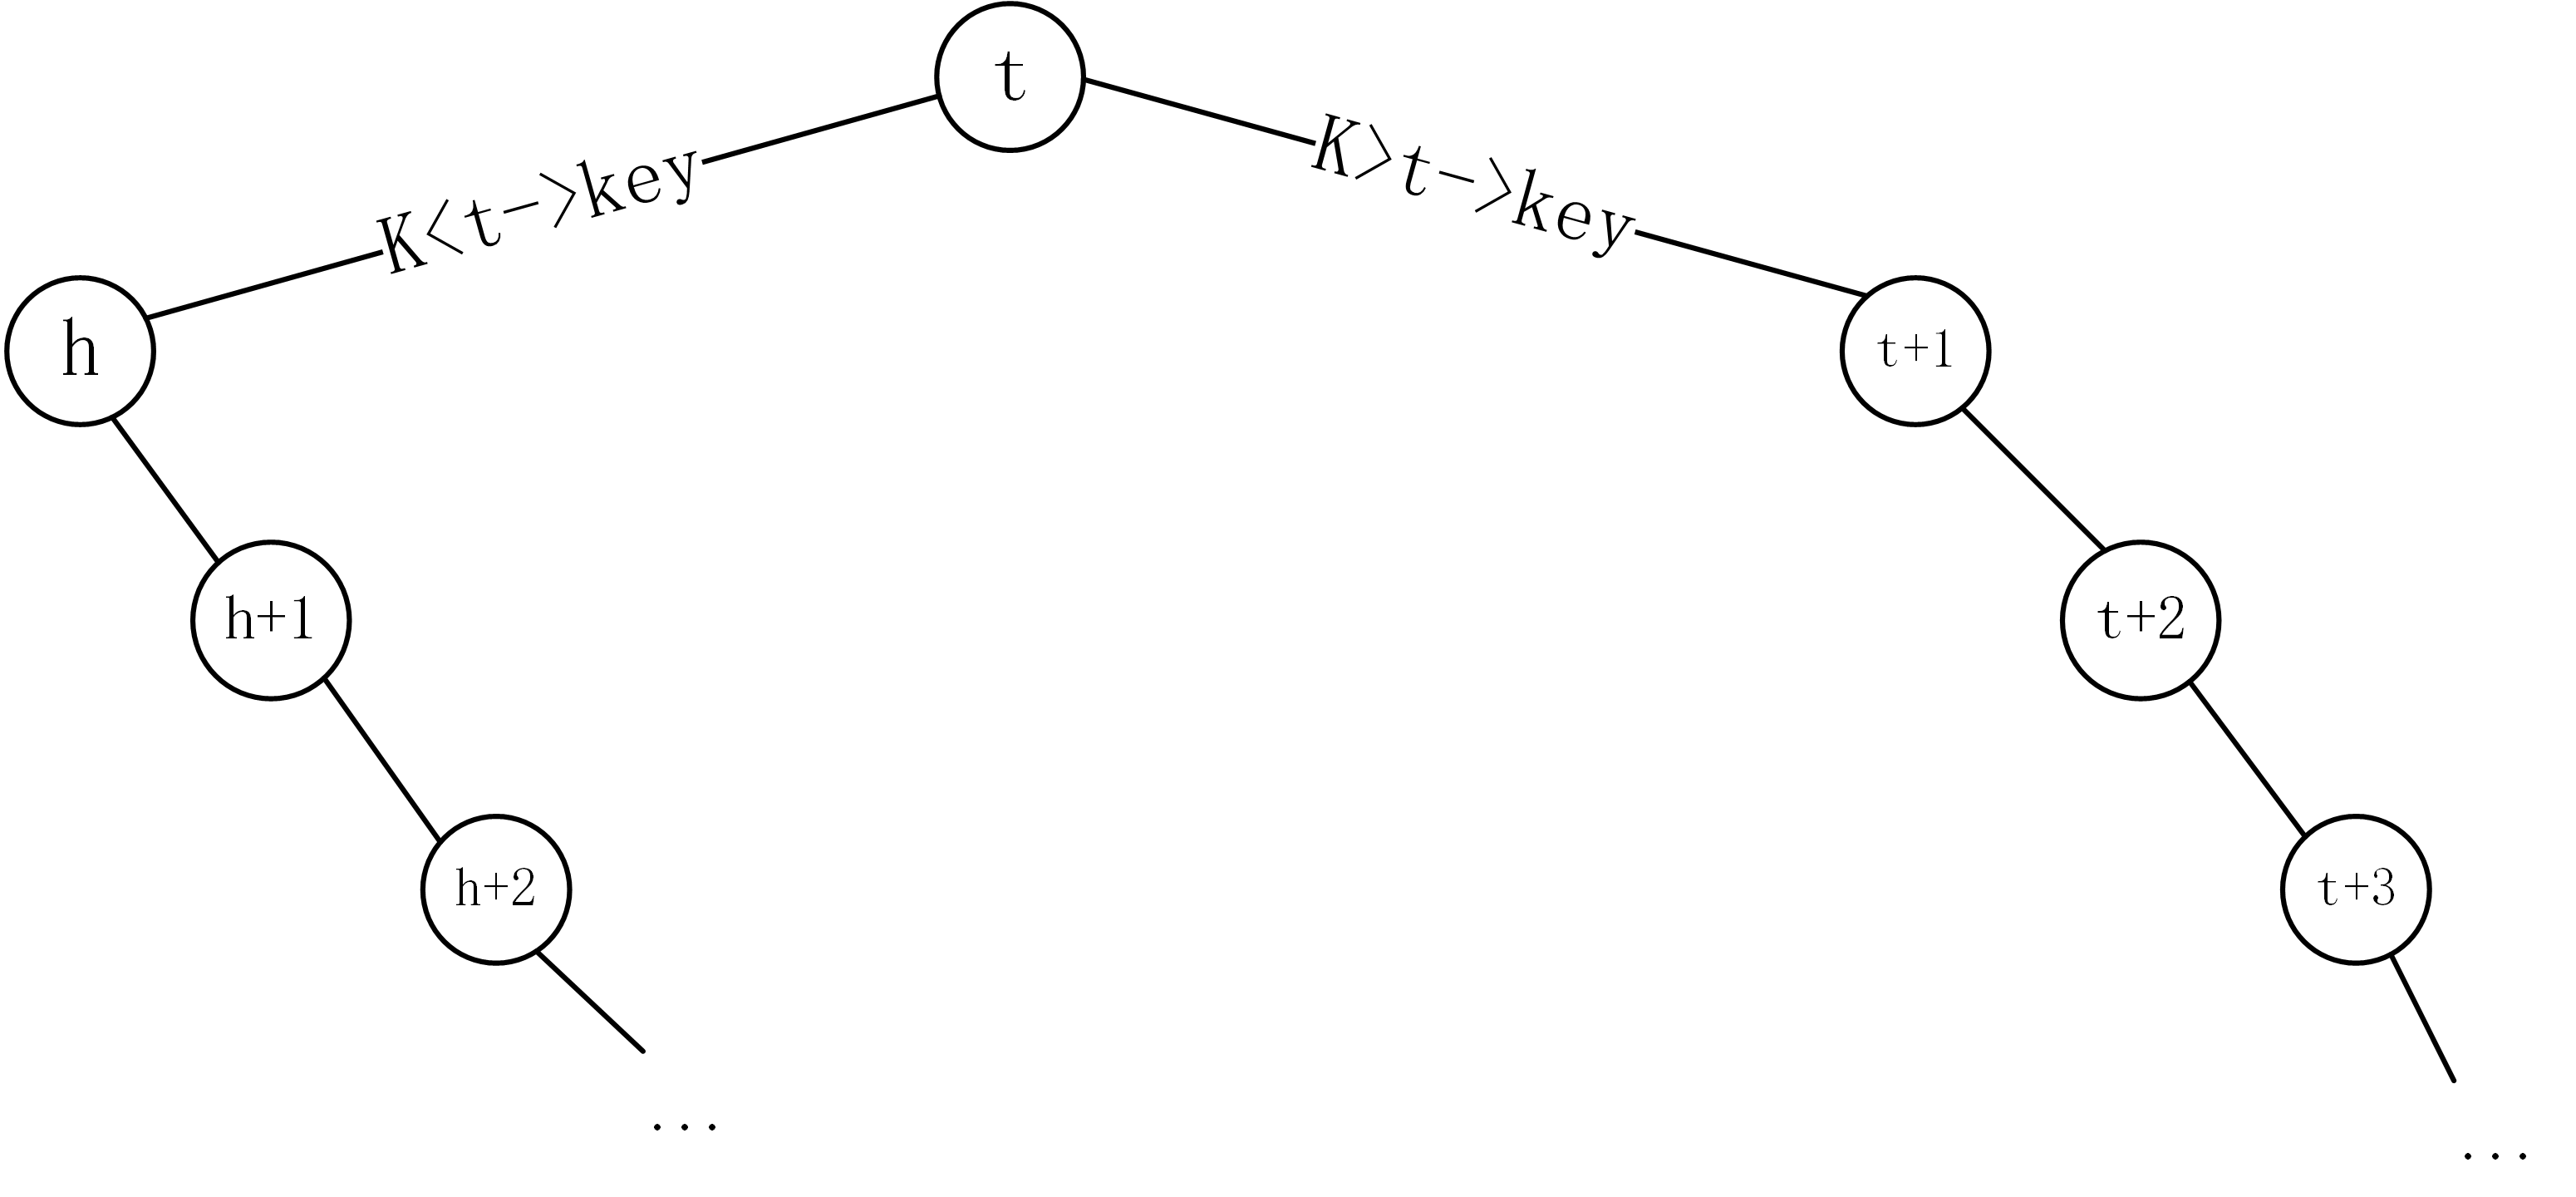
\includegraphics[scale=1]{9-29.png}\\
平均查找长度分析:\\
设f(i,j)函数为t=i,k=j时的概率,则有$f(i,j)=\frac{1}{n^2}$
则对每种情况的查找长度分为一下几种情况:
$$
L(i,j)=
\left\{
    \begin{aligned}
        &j+1,~~j<i\\
        &1,~~j=i\\
        &j-i+1,~j>i~and~j<n
    \end{aligned}
\right.
$$
则平均查找长度为:
$$
\begin{aligned}
&\sum \sum f(i,j)L(i,j)\\
&=\sum_{i=1}^{n} \sum_{j=1}^{i-1} \frac{j+1}{n^2}+1+\sum_{i=1}^{n} \sum_{j=i+1}^{n} \frac{j-i+1}{n^2}\\
&=\frac{n^3+6n-4}{3n^2}
\end{aligned}
$$
因此平均查找时间复杂度为$O(\frac{n}{3})$。\\[1cm]
\textbf{9-35}\\
假设二叉排序树以后继线索链表作存储结构,编写输出该二叉树中所有大于a并且小于b的关键字的算法。\\
\textbf{算法分析}\\
若要形成排序线索树,那么应该按照中序线索树建造线索,并且支持动态插入,当有一个询问时,调用search函数进行中序遍历(线索)查询。\\
时间复杂度O(logn)(平衡二叉树),O(n)(普通二叉树,取决于插入顺序),空间复杂度O(n)。
\textbf{code}
\begin{lstlisting}
    #include<bits/stdc++.h>
    #define maxn 1000
    using namespace std;
    struct node
    {
        int num;
        node * lson;
        node * rson;
    };
    int n,m;
    void insert(int x,node *hp)
    {
        if (x<hp->num)
        {
            if (hp->lson!=NULL) 
            {
                insert(x,hp->lson);
                return;
            }
            else 
            {
                node*p1=(node *)malloc(sizeof(node));
                hp->lson=p1;
                p1->lson=NULL;p1->rson=NULL;
                p1->num=x;
                return;
            }
        }
        else
        {
            if (hp->rson!=NULL)
            {
                insert(x,hp->rson);
                return;
            }
            else 
            {
                node*p1=(node *)malloc(sizeof(node));
                hp->rson=p1;
                p1->lson=NULL;p1->rson=NULL;
                p1->num=x;
                return;
            }
        }
    }
    void search(node *hp,int Min,int Max)
    {
        if (hp->lson!=NULL) 
            search(hp->lson,Min,Max);
        if (hp->num>=Min && hp->num<=Max) 
            cout<<hp->num<<" ";
        if (hp->rson!=NULL)
            search(hp->rson,Min,Max);
    }
    void init()
    {
        cout<<"please input the number:"<<endl;
        cin>>n;
        int a;
        node *h=(node *)malloc(sizeof(node));
        h->lson=NULL;
        h->rson=NULL;
        cin>>h->num;
        for (int i=1;i<n;i++)
        {
            cin>>a;
            insert(a,h);
        }
        cout<<"please input the query number:"<<endl;
        cin>>m;
        for (int i=0;i<m;i++)
        {
            int A,B;
            cin>>A>>B;
            search(h,A,B);
            cout<<endl;
        }
    }
    int main()
    {
        init();
    }    
\end{lstlisting}
textbf{9-38}\\
试写一个算法,将两个排序二叉树合并为一个排序二叉树。\\
textbf{算法分析}\\
1.将结点少的树拆散一个个插入另外一棵树,时间复杂度O(nlogn)(平衡二叉树),空间复杂度O(n)。\\
2.同时中序遍历两颗二叉树的同时建立另外一棵树,设立两个指针指向两树的当前结点。\\
时间复杂度O(N),空间复杂度O(N).
\text{code}
\begin{lstlisting}
    #include<bits/stdc++.h>
    using namespace std;
    typedef struct BinNode
    {
        int data;
        struct BinNode *lchild;
        struct BinNode *rchild;
    }BinNode,*BinTree;
     
    void CreateBinTree(BinTree *tree)
    {
        int val;
        scanf("%d",&val);
        if(val==-1)
        {
            (*tree)=NULL;
        }
        else
        {
            *tree=(BinTree)malloc(sizeof(BinNode));
            (*tree)->data=val;
            CreateBinTree(&((*tree)->lchild));
            CreateBinTree(&((*tree)->rchild));
        }
    }
     
    void Inorder(BinTree T)
    {
        if(T)
        {
            Inorder(T->lchild);
            printf("%d ",T->data);
            Inorder(T->rchild);
        }
    }
     
    void Insert(BinTree *T,int key)
    {
        if(!(*T))
        {
            (*T)=(BinTree)malloc(sizeof(BinNode));
            (*T)->data=key;
            (*T)->lchild=(*T)->rchild=NULL;
            return;
        }
        if(key==(*T)->data)
            return;
        if(key>(*T)->data)
            Insert(&((*T)->rchild),key);
        else
            Insert(&((*T)->lchild),key);
    }
     
    void InsertBST(BinTree T1,BinTree T2)
    {
        if(T2)
        {
            InsertBST(T1,T2->lchild);
            Insert(&T1,T2->data);
            InsertBST(T1,T2->rchild);
        }
    }
     
    int main()
    {
        BinTree T1=NULL;
        BinTree T2=NULL;
        CreateBinTree(&T1);
        CreateBinTree(&T2);
        InsertBST(T1,T2);
        Inorder(T1);
        printf("\n");
        return 0;
    }
\end{lstlisting}
\textbf{9-40}\\
在平衡二叉树的每个结点增设一个lsize域,其值为它左子树的结点数+1,试写一个时间复杂度为O(logn)的算法,确定树中的第k小结点的位置。\\
\textbf{算法分析}\\
利用中序遍历现初始化setup left(lsize域),当有询问k时,直接一层层比较,向叶子结点递归即可。由于树高度不超过logn+1\\
时间复杂度O(logn),空间复杂度O(n).
\begin{lstlisting}
    #include<bits/stdc++.h>
    #define maxn 1000
    using namespace std;
    struct node
    {
        int num;
        node * lson;
        node * rson;
        node * fa;
        int left;
    };
    int n,m;
    bool flag;
    int number;
    void insert(int x,node *hp)
    {
        if (x<hp->num)
        {
            if (hp->lson!=NULL) 
            {
                insert(x,hp->lson);
                return;
            }
            else 
            {
                node*p1=(node *)malloc(sizeof(node));
                hp->lson=p1;
                hp->left=0;
                p1->lson=NULL;p1->rson=NULL;p1->fa=hp;
                p1->num=x;
                return;
            }
        }
        else
        {
            if (hp->rson!=NULL)
            {
                insert(x,hp->rson);
                return;
            }
            else 
            {
                node*p1=(node *)malloc(sizeof(node));
                hp->rson=p1;
                hp->left=0;
                p1->lson=NULL;p1->rson=NULL;p1->fa=hp;
                p1->num=x;
                return;
            }
        }
    }
    void search(node *hp,int Min,int Max)
    {
        if (hp->lson!=NULL) 
            search(hp->lson,Min,Max);
        if (hp->num>=Min && hp->num<=Max) 
            cout<<hp->num<<" ";
        if (hp->rson!=NULL)
            search(hp->rson,Min,Max);
    }
    void setup(node *hp,int k)
    {
        if (hp->lson!=NULL)
            setup(hp->lson);
            number++;
            hp->left=number;
            if (hp->left==k)
        if (hp->rson!=NULL)
            setup(hp->rson);
    }
    void del(node *hp,int inx)
    {
        if (flag) return;
        if (inx<hp->num)
            del(hp->lson,inx);
        if (inx>hp->num)
            del(hp->rson,inx);
        if (inx==hp->num)
            {
               flag=true;
               if  (hp->lson==NULL)
               {
                   hp->lson->fa=hp->fa;
                   if (hp->fa->lson==hp)
                       hp->fa->lson=hp->rson;
                   if (hp->fa->rson==hp)
                       hp->fa->rson=hp->rson;
               }
               if (hp->lson!=NULL)
               {
                    node*p1=hp->lson;
                    if (p1->rson==NULL)
                    {
                        hp->lson->fa=hp->fa;
                        if (hp->fa->lson==hp)
                            hp->fa->lson=hp->lson;
                        if (hp->fa->rson==hp)
                            hp->fa->rson=hp->lson;
                            hp->lson->rson=hp->rson;
                            hp->rson->fa=hp->lson;
                    }
                    else
                    {
                        while(p1->rson!=NULL)
                            p1=p1->rson;
                        p1->fa->rson=p1->lson;
                        p1->lson->fa=p1->fa;
                        p1->lson=hp->lson;
                        p1->rson=hp->rson;
                        p1->fa=hp->fa;
                        if (hp->fa->lson==hp)
                            hp->fa->lson=p1;
                        if (hp->fa->rson==hp)
                            hp->fa->rson=p1;
                        hp->rson->fa=p1;
                        hp->lson->fa=p1;
                    }
                    free(hp);
               }
            }
        return;
    }
    void init()
    {
        cout<<"please input the number:";
        cin>>n;
        int a;
        node *root=(node *)malloc(sizeof(node));
        node *h=(node *)malloc(sizeof(node));
        h->lson=NULL;
        h->rson=NULL;
        h->fa=root;
        cin>>h->num;
        for (int i=1;i<n;i++)
        {
            cin>>a;
            insert(a,h);
        }
        cout<<"please input the query number:";
        cin>>m;
        for (int i=0;i<m;i++)
        {
            int A;
            cin>>A;
            setup(h,A);
        }
    }
    int main()
    {
        init();
    }
\end{lstlisting}
\end{document}